% This is samplepaper.tex, a sample chapter demonstrating the
% LLNCS macro package for Springer Computer Science proceedings;
% Version 2.20 of 2017/10/04
%
\documentclass[runningheads]{llncs}
%

% Setup packages
\usepackage{booktabs}
\usepackage{graphicx}
\usepackage{multicol}
\usepackage[T1]{fontenc}
\usepackage[utf8]{inputenc}
\usepackage{float}
\usepackage{babel}
\usepackage{subcaption}
\usepackage{graphicx}
\usepackage{appendix}
\usepackage{caption}



% Used for displaying a sample figure. If possible, figure files should
% be included in EPS format.
%
% If you use the hyperref package, please uncomment the following line
% to display URLs in blue roman font according to Springer's eBook style:
% \renewcommand\UrlFont{\color{blue}\rmfamily}

\pagenumbering{arabic}

\graphicspath{ {media/} } 

\begin{document}


\title{Contribution Title\thanks{Supported by organization x.}}
%
%\titlerunning{Abbreviated paper title}
% If the paper title is too long for the running head, you can set
% an abbreviated paper title here
%
\author{First Author\inst{1}\orcidID{0000-1111-2222-3333} \and
Second Author\inst{2,3}\orcidID{1111-2222-3333-4444} \and
Third Author\inst{3}\orcidID{2222--3333-4444-5555}}
%
\authorrunning{F. Author et al.}
% First names are abbreviated in the running head.
% If there are more than two authors, 'et al.' is used.
%
\institute{Princeton University, Princeton NJ 08544, USA \and
Springer Heidelberg, Tiergartenstr. 17, 69121 Heidelberg, Germany
\email{lncs@springer.com}\\
\url{http://www.springer.com/gp/computer-science/lncs} \and
ABC Institute, Rupert-Karls-University Heidelberg, Heidelberg, Germany\\
\email{\{abc,lncs\}@uni-heidelberg.de}}
%
\maketitle              % typeset the header of the contribution
%
\begin{abstract}
Prior to elections viewpoints of parties and individual users  are often expressed on Social Networking Sites (SNS) since expressing opinition is one of the core characteristics of social media. Recently, (November 2023) elections for the Dutch House of Representatives took place. This study focuses on on a data-driven social web approach aiming to answer the research question: \textit{to what extent is the relatively new SNS Mastodon representative of the election voting of the dutch population?} In the analysis this research processed data from several election-related resources such as political parties and topics from election manifestos and are cross-referenced and statistically analysed with Mastodon instance-wide (e.g. servers) and Streaming API (e.g. toots and mentions). The results indicated that there is a significant increase in activity related to the dutch election on the Mastodon platform and political parties and candidates are increasingly creating user accounts and instances. Privacy and ethical considerations when accessing Mastodon platform data are discussed and in the future work section, the study addresses several further enhancement that can be performed to automate more of the processing methods and to further expand the election data sources used.

\keywords{Social Web  \and Social Network \and Network Analysis \and Mastodon \and Dutch Elections \and Political Parties \and User-generated Content.}
\end{abstract}
\section{Introduction}

In order to investigate this social web related topic, this study aims to answer the research question:
\textbf{\textit{"To what extent is the relatively new Social Networking Site Mastodon representative of the election voting of the dutch population?"}}. To answer this research question in-depth, the following sub-questions were formulated:

\begin{itemize}
  \item \textbf{R1:} \textit{What's the distribution of political parties on the platform and do they align with the outcome of the election? }
  \item \textbf{R2:} \textit{What political topics are discussed in posts and are they representative of the election manifesto of political parties? }
  \item \textbf{R3:} \textit{Do the topics that are discussed on the platform align with popular voting guides?}
\end{itemize}

The sub-questions are relevant to the main research question as they provide a more detailed and specific understanding of the topic. For our research we use Mastodon as a Social Networking site (SNSen) as case study and main data source but this research can be further expanded to any social network if the platform has an API that exposes platform data and has the characteristics of a typical social network. To check, validate and cross-reference our sub-questions we complement this data with three additional data sources: 

\begin{itemize}
  \item \textbf{Institut Public de Sondage d'Opinion Secteur (IPSOS) exitpoll:} a market research company which, commisioned by the 'Nederlandse Omroep Stichting' \footnote{https://nos.nl/} (NOS; English: Dutch Broadcasting Foundation) publishes market research about the elections (e.g. which voters switch between parties, which municipilaties has switched the most between parties) \cite{nos}.
  \item \textbf{Government Open Data (overheid.nl)}: specifically the datasets from The Dutch Electoral Council \footnote{https://www.kiesraad.nl/} (Dutch: Kiesraad), the government body that is responsibly for counting of the votes and publishing the results \cite{kiesraad}.
  \item \textbf{ProDemos voting guide (stemwijzer)}: a voting guide called Stemwijzer \footnote{https://home.stemwijzer.nl/} with pre-defined topics. By answering 30 statements with agree, disagree or no opinion, voters can compare their positions with those of political parties. Many of these voting guides exist, ProDemos is most requested and partly funded by the dutch government \cite{prodemos}.
\end{itemize}

\section{Related Work}

Social networking sites and other popular online platforms have been used as a means to express political opinions and show support and/or dissent for particular political parties or ideologies quite regularly during election periods since the rise of social media. Citizens are able, thanks to social media, to follow politicians, political commentators and political consultants as a way to spread messages of endorsement and opposition through the sharing and posting of digital content; this phenomenon known as 'political advertising' took place even before the rise of social media and allowed for properly structured campaign advertisements to take place on digital platforms (https://blog.oup.com/2017/06/history-political-social-media/) As a matter of fact, as well as  political opinions and views provided by individual users or voters, political parties use these platforms and the underlying channels of communication to run their political campaigns and thus, draw further attention for political debate and discourse. 

Since the officially recorded use of social media for political campaigns, with Barack Obama's electoral campaign run in 2008, until current times, social media has been one of the primary political ideology battlefields across the globe, optimally leveraging the growing number of social media users and consequently that of people eligible to vote. (https://journals.sagepub.com/doi/10.1177/20563051211063461) This incremental evolution saw a deeper and more analytical organization of campaigns and political discourse on social media platforms effectively making these platforms key players in the domain of digital political journalism. (Kreiss D. (2012). \textit{Taking our country back: The crafting of networked politics from Howard Dean to Barack Obama}. Oxford University Press.)

Consequently, online political discourse through digital platforms became 


\section{Methodology}

\subsection{Data collection (datasets)}

To gather social web data from Mastodon the official public Mastodon API \footnote{https://docs.joinmastodon.org/client/intro/} using the Mastodon.py \footnote{https://mastodonpy.readthedocs.io/en/stable/}wrapper for Python is used. Mastodon is an ActivityPub-based \footnote{https://www.w3.org/TR/activitypub/} Twitter-like federated social network node. The API wrapper is feature complete for Mastodon the Mastodon API version 3.5.5. First a user account is created on the platform by completing the sign-up for an account flow on the Mastodon official website \textit{joingmastodon.org}. The account is created on the general and largest public server (provider) \textit{mastodon.social} operated by the Mastodon gGmbH non-profit.

To interact with the Mastodon servers through Python using the Mastodon.py wrapper an application registration is performed which gives a client key and client secret to allow logging in and accessing API data using access tokens. For this research we mainly used API methods for:

\begin{itemize}
  \item \textbf{Accounts, relationships and lists:} allows for geting information about accounts and associated data as well as update that data
  \item \textbf{Instance-wide data and search:}  fetch information associated with the current instance as well as data from the instance-wide profile directory
  \item \textbf{Streaming:} allow access to the streaming API. For the public, local and hashtag streams,
\end{itemize}

Arguments and parameters used in functions written for the Mastodon API methods are related to the dutch elections (e.g. names of political candidates, popular topics from parties) further expanded upon in the data preprocessing and results section of this research. To check, validate and cross-reference the sub-questions the data is complementend with five additional election related data sources: 

\begin{itemize}
  \item \textbf{Institut Public de Sondage d'Opinion Secteur (IPSOS) exitpoll:} a market research company which, commisioned by the 'Nederlandse Omroep Stichting' \footnote{https://nos.nl/} (NOS; English: Dutch Broadcasting Foundation) publishes market research about the elections (e.g. which voters switch between parties, which municipilaties has switched the most between parties) \cite{nos}. This gives a comprehensive insight of voting behaviour from the recent election.
  \item \textbf{Government Open Data (overheid.nl)}: specifically the datasets from The Dutch Electoral Council \footnote{https://www.kiesraad.nl/} (Dutch: Kiesraad), the government body that is responsibly for counting of the votes and publishing the results \cite{kiesraad}. This gives the official results of parties and candidates from the recent elections.
  \item \textbf{ProDemos voting guide (stemwijzer)}: a voting guide called Stemwijzer \footnote{https://home.stemwijzer.nl/} with pre-defined topics. By answering 30 statements with agree, disagree or no opinion, voters can compare their positions with those of political parties. Many of these voting guides exist, ProDemos is most requested and partly funded by the dutch government \cite{prodemos}. This gives insight in important topics from political parties for the recent elections.
  \item \textbf{Electoral Council (kiesraad)}: the Kiesraad \footnote{https://english.kiesraad.nl/} is a central electoral committee, an advisory body and acts as a central polling station during the dutch house of representatives election. For this research we used the published Candidacy for the House of Representatives election list and the Political Party Registrar.
  \item \textbf{Netherlands Bureau for Economic Policy Analysis (cpb)}: the dutch economics bureau (CPB) \footnote{https://www.cpb.nl/en/charted-choices-2025-2028} performs election manifestos analysis to determine how feasible manifestos of political parties are. This gives an overview of topics that are in the election manifestos of political parties.
\end{itemize}

\subsection{Data preprocessing (scope)}

- Timeline from previous elections 2019. \\
- Only 'sitting' parties. There are more parties in total. \\
- Synonyms from parties, abbreviations etc. \\

Each of the parties is placed on a political spectrum (left, lean left, center, lean right, righ). Quote a source. There is probably an 'official' list for this. Based on what they voted (maybe stemmentracker)? \\

Here a table of all parties? If they are left-wing, right-wing. How many zetels.



\subsection{Data analysis}

Write here about how we analyzed data. Using python, networkX etc. notebooks. What we automated, what we did manually.
\section{Results}
The results section is divided into three subsections, each corresponding to the individual research questions as described in the \textit{introduction} section. (R1) Relateing to activity of political parties on the platform, (R2) relating to topics from election manifestos and voting guides, and (R3) relating to a network analysis of instances and servers of political parties on the network. Each with accompanying descriptions of the methods performed and graphs to further understand the data and the result of the analysis.

A clear increase in general activity surrounding the Dutch elections on the platform is found.
When querying toots with general terms on Dutch elections, for example “verkiezingen”, “ducth elections”, or “tweede kamer”, the results have very clearly spiked in the last period, as shown in figure \ref{fig:electionstotal}. A total of 18,230 toots were retrieved, which included these election related terms, of which around 16,000 are in the last two years.
Therefore, Mastodon has been more widely adopted for the most recent election year, 2023, as opposed to previous elections, 2017 and 2021, which showed almost no activity on these general queries.

\begin{figure}[ht]
  \centering
  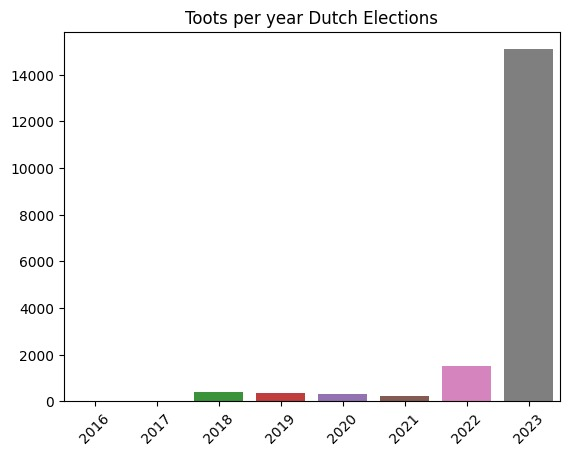
\includegraphics[width=3.25in]{media/dutch-elections-mastodon.jpeg}
  \caption{Bar chart of query word results, using general terms surrounding Dutch elections}
  \label{fig:electionstotal}
\end{figure}

\subsection{Activity of Political Parties (R1)}
With the list of terms extracted from the voting guide, the platform is queried for these terms and cross-referenced with party names, resulting in a dataset reflecting what parties get mentioned most topically on Mastodon.
The resulting graph in figure \ref{fig:partymentions} makes it clear that the Dutch socialist party (SP) is mentioned in conjunction with the topical terms the most.
The candlestick graph, where the wick represents the deviation of terms, shows that the SP also has the widest variety of topics mentioned.
One possible explanation is that their party initials are found in Dutch spelling quite commonly.
However, when isolation their initials, the results are the same, although this could still be the result of errors in our search endpoint syntax.
It is safe to assume the SP is an outlier, considering the second-highest activity party, is active on the platform itself and has a separate Mastodon instance

\begin{figure*}[ht]
  \centering
  \begin{subfigure}[h]{.49\linewidth}
    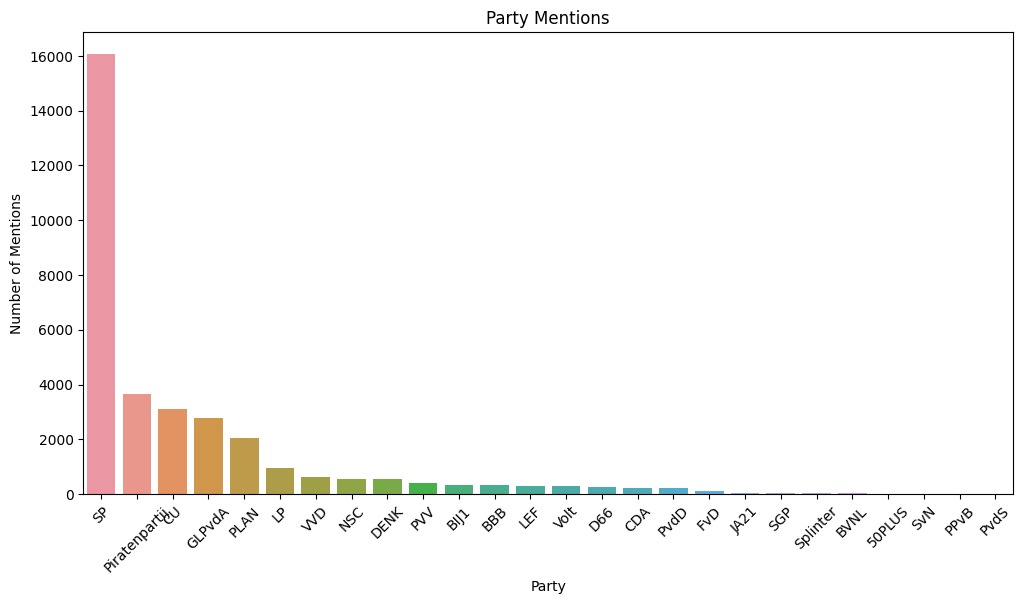
\includegraphics[width=\textwidth]{media/party-mentions.jpeg}
    \captionsetup{justification=centering}
    \caption{Bar chart showing individual political party mentions}
    \label{fig:partymentions}
  \end{subfigure}
  \begin{subfigure}[h]{.49\linewidth}
      \captionsetup{justification=centering}
      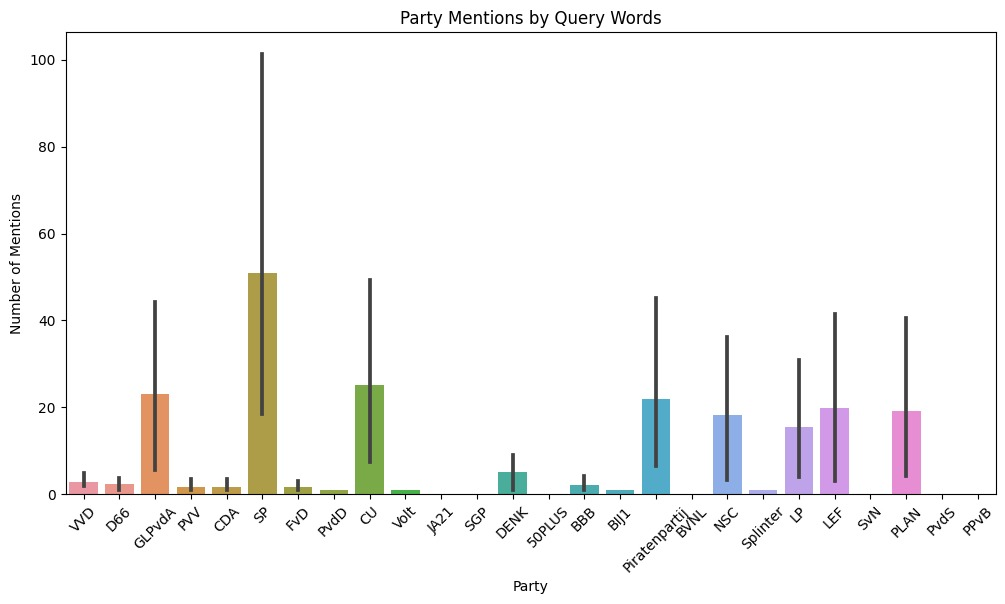
\includegraphics[width=\textwidth]{media/party-mentions-query-words.jpeg}
      \caption{Candlestick chart showing parties being mentioned based on topical query words. The wick represents the spread of unique topics}
      \label{fig:partycandle}
  \end{subfigure}
  \caption{Graphs visualizing party activity based on party name mentions and query words based on topics}
  \label{fig:results}
\end{figure*}

Activity around parties seems to focus around a small set of parties.
The second-highest mention, which seems like a more realistic activity hotspot, is the piratenpartij.
Piratenpartij has its own Mastodon instance and multiple accounts, which also have the most activity itself, when compared to other party account on the platform, more in this is shown in the subsection for (R3).
Their deviation in figure \ref{fig:partycandle} also shows they are talked about in conjunction with a wide variety of topics.
Interestingly, the GL-PvdA party comes very close to the piratenpartij, even though they are not active on the platform themselves.
An easy explanation would be, that this party has a lot of young voters and was mentioned in passing quite often because of their fusion (they used to be two separate parties).
Moreover, a large group of their constituents is known to be active in online discourse on other social media as well, as well as the sister party of the SP aimed at teenagers. 

\textbf{Finding M1:} \textit{Very few parties get mentioned, however, the parties that are mentioned are actively discussed. The cross-referencing might be influenced by the prevalence of the initials of parties in the Dutch language.}

\subsection{Election-related topics and query words (R2)}
The related topics mentioned per party mention shows an interesting spread when plotted.
A hot topic, reasonably, is climate (and climate change) and “economy”, which in hindsight, might have been too general of a term, that etymologically contains most other terms as well.
These topics get mentioned almost exclusively by left leaning parties, although it must be noted that almost all parties that have a reasonable amount of activity are left leaning.
When comparing this chart to the activity around parties, it becomes clear there are certain queries that result in actual political discourse toots and queries that don't really have that much activity.
Most mentions group around the active parties, while other mentions are so sparse and distributed, it seems more like the discourse is somewhat evenly spread across topics, when the party and topic itself get mentioned by users.
There is no clear distinction in actual difference of discourse between parties.
\begin{figure}[ht]
  \centering
  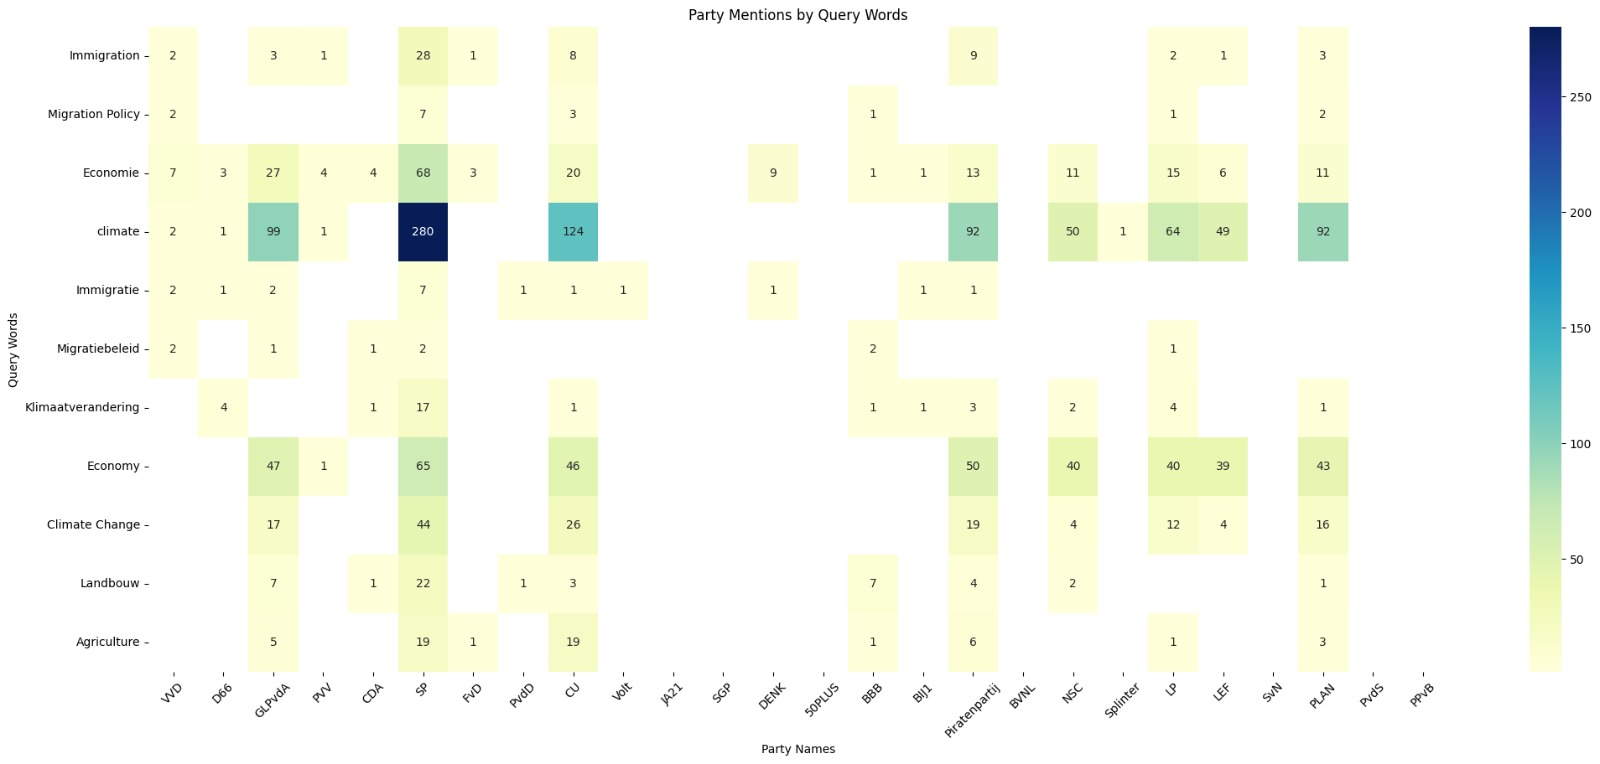
\includegraphics[width=\linewidth]{media/party-mentions-topics.jpeg}
  \caption{Party mentions related to topics}
  \label{fig:topic}
\end{figure}


\textbf{Finding M2:} \textit{Overall discourse seems to be on similar topics, only showing up in searches surrounding parties that have activity on the platform}

\subsection{Analysis of Party accounts and servers (R3)}
To more easily convey what parties have adopted the network, multiple queries have been performed, and analysed to find accounts connected to parties.
A list of all parties, including their nicknames and different spellings of abbreviations or of those nicknames is looped through and queried in conjunction with different terms like “official”, “party”, “House of Representatives”, or “elections”, albeit in Dutch.
These queries resulted in the tree of different party accounts, as seen in figure \ref{fig:partynetwork}.

Noticeably, there are some parties that are not active on the main server, but instead have made their own server.
The piratenpartij and Bij1 both have their own server, where the piratenpartij server is actually quite active, at least compared to Bij1's server.
This also does not surprise from a political point of view, as the piratenpartij, translated to pirate party, was founded to legislate in internet laws and protect net neutrality.
The self-proclaimed radical left Bij1 party also occasionally mentions their need to operate in decentralized structures and hierarchies in their news and SNS outings.
The distinction between servers is more easily seen in figure \ref{fig:servernetwork} which branches to parties starting from the server as opposed to branching off from the party.

\begin{figure}[ht]
  \centering
  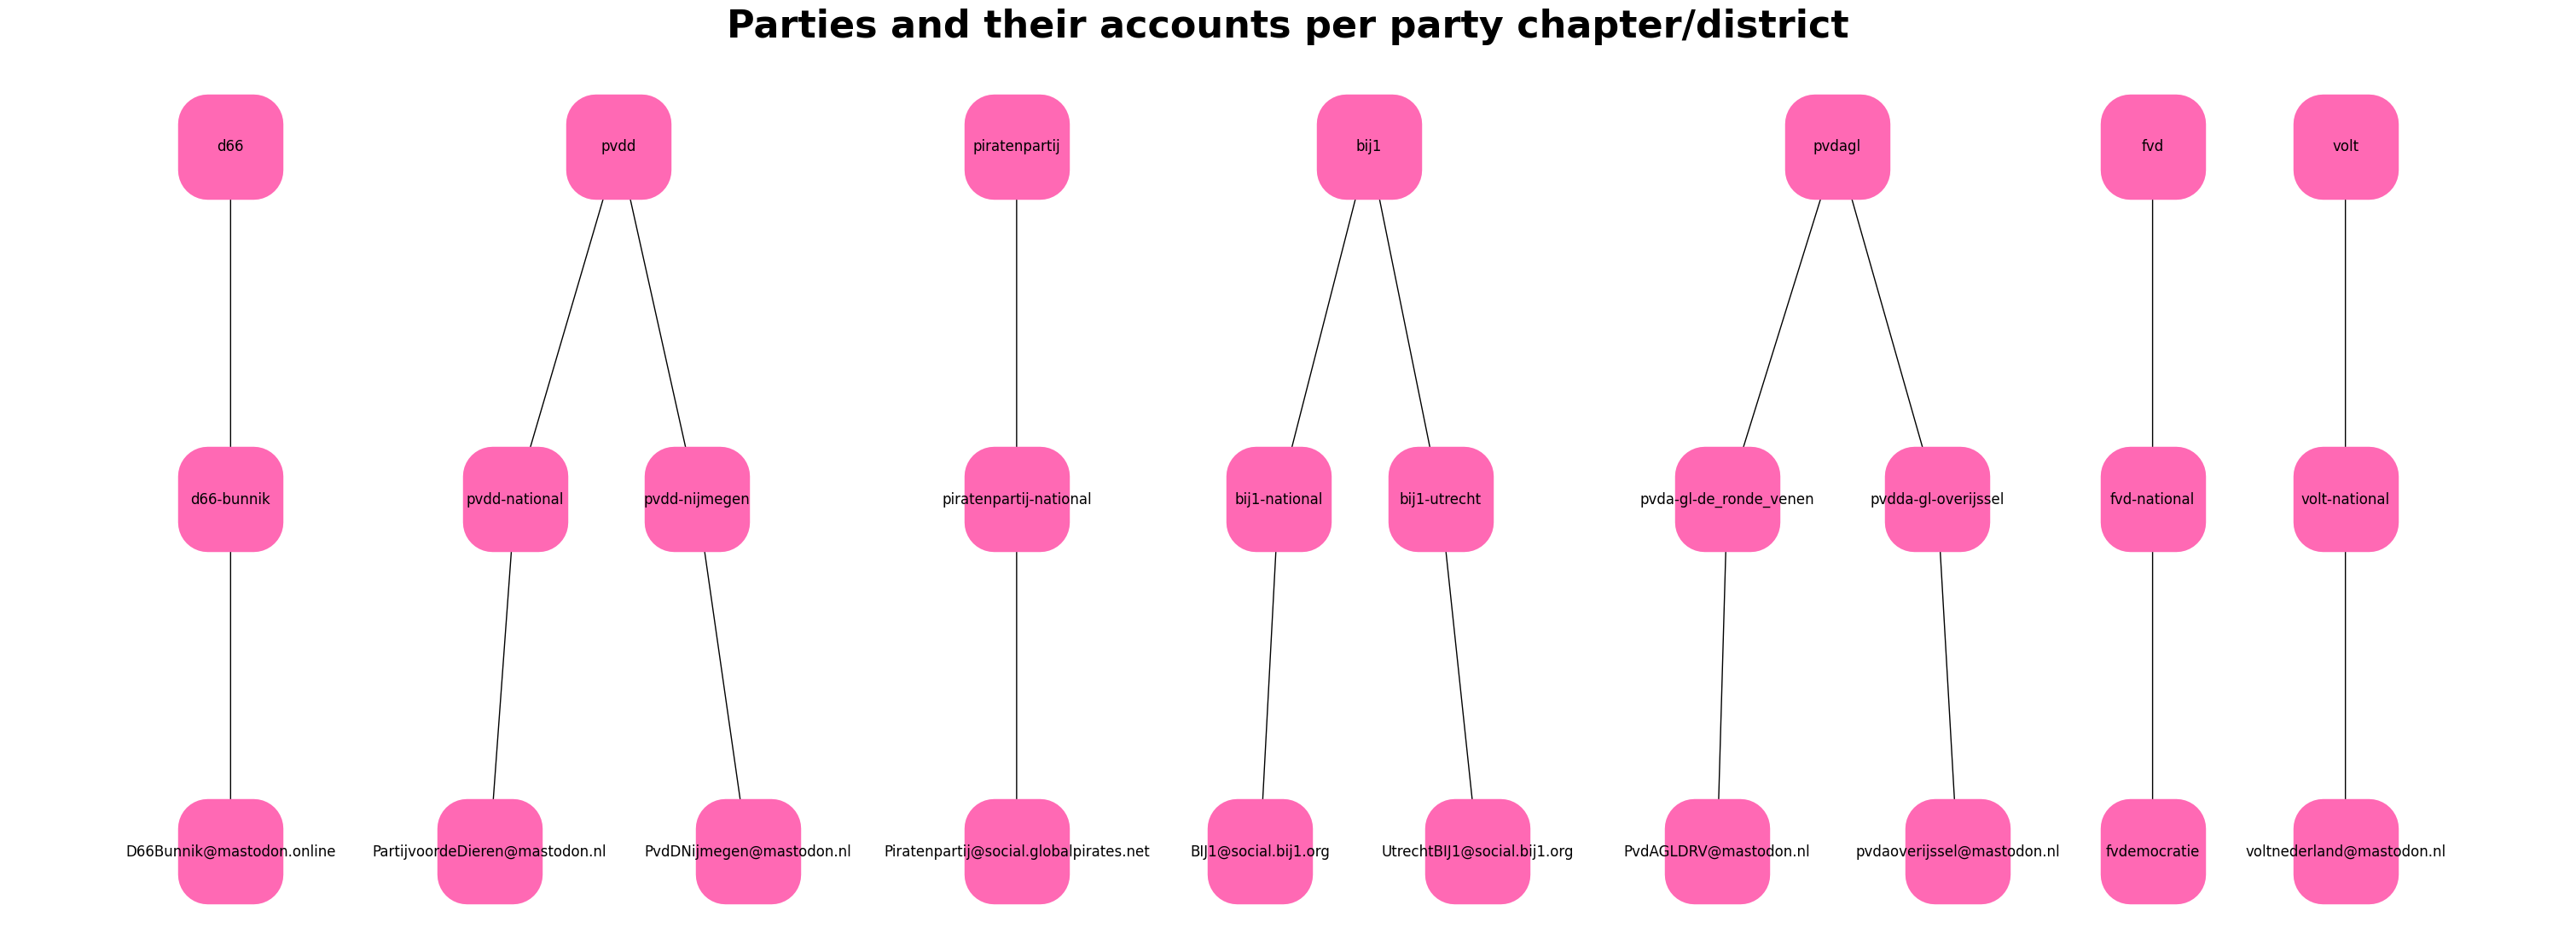
\includegraphics[width=\linewidth]{media/chapter.png}
  \caption{Tree of party accounts, branching from their district}
  \label{fig:partynetwork}
\end{figure}

\begin{figure}[ht]
  \centering
  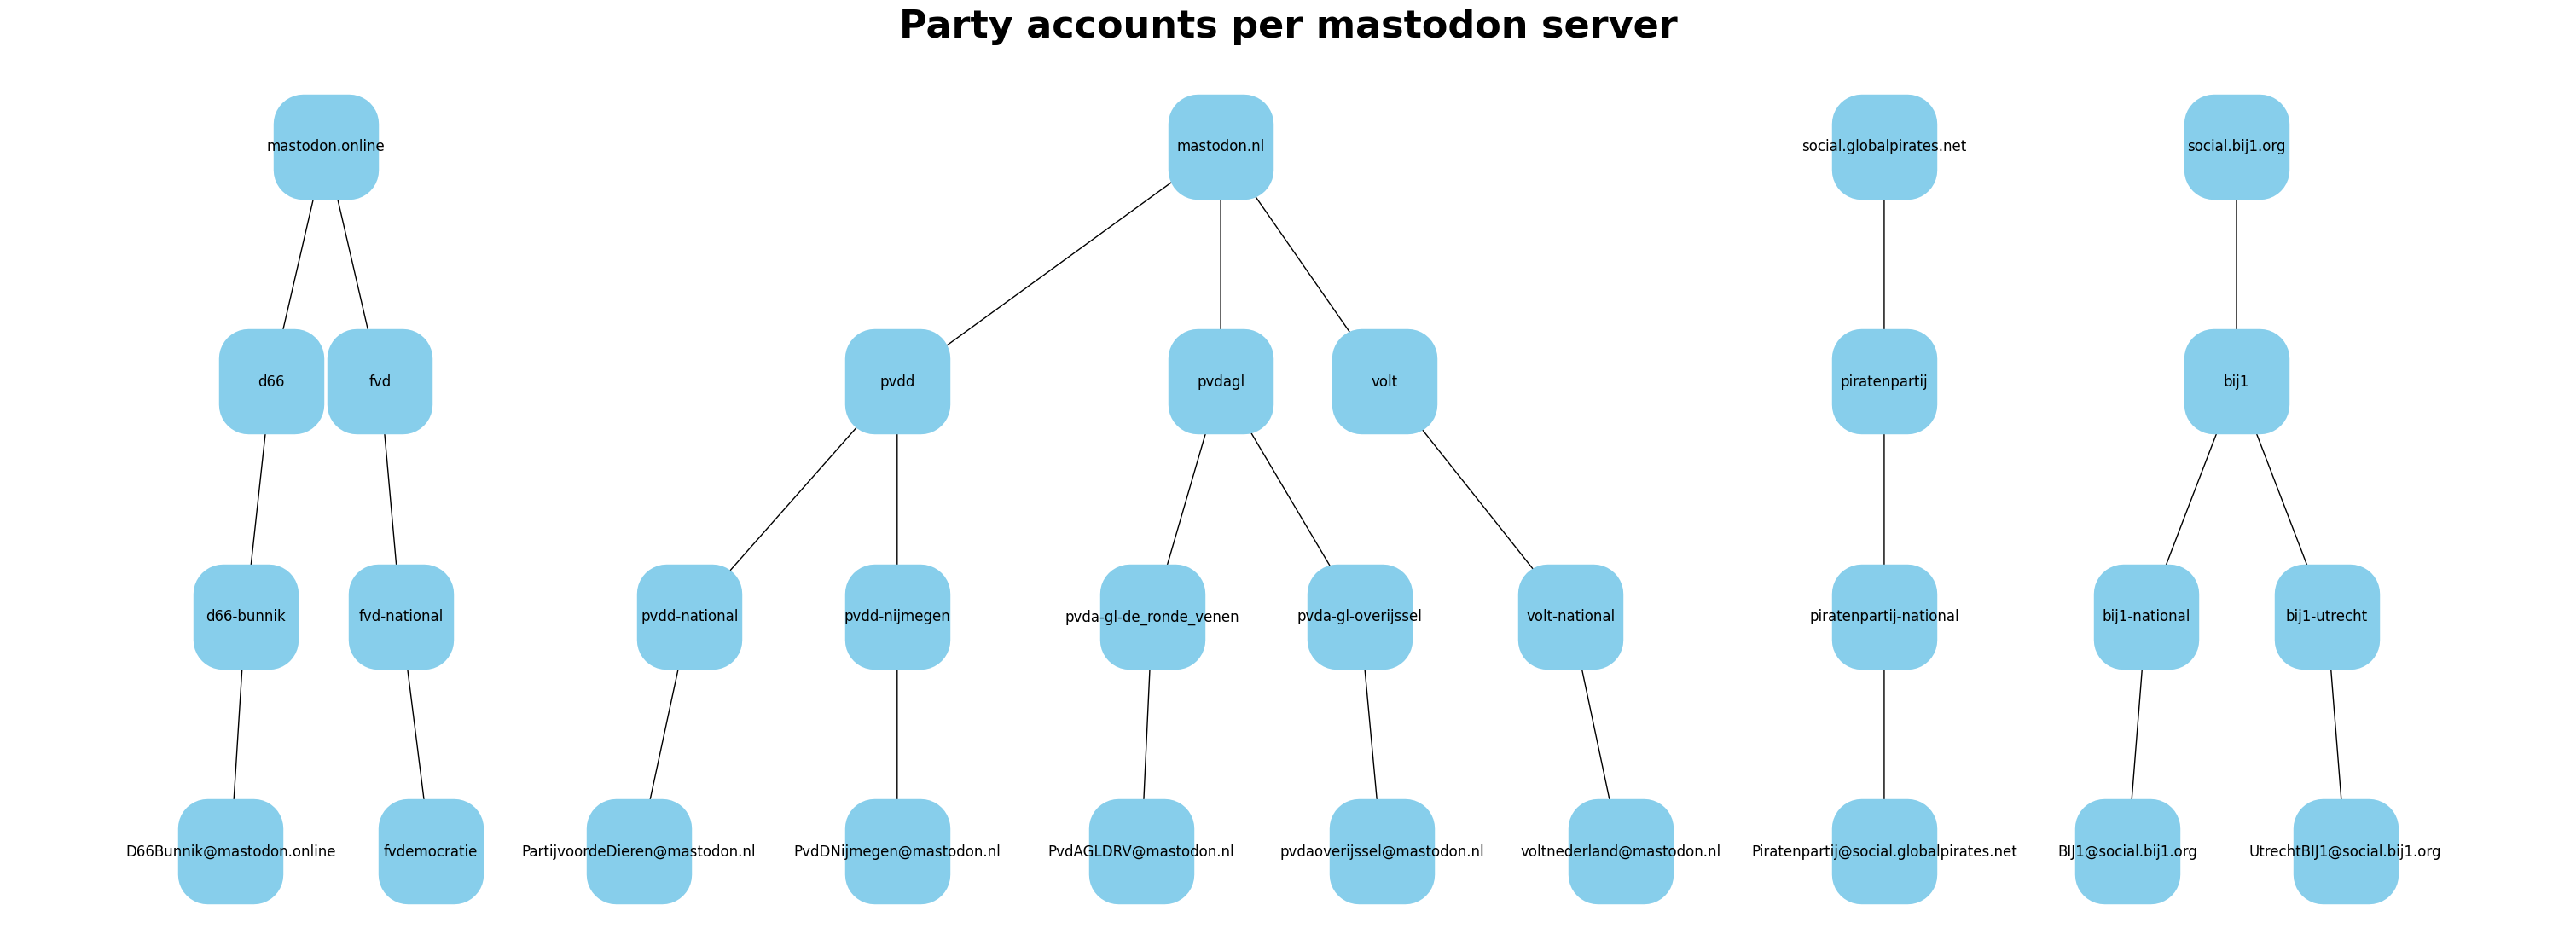
\includegraphics[width=\linewidth]{media/server.png}
  \caption{Tree of party accounts, branching from their respective server}
  \label{fig:servernetwork}
\end{figure}

\begin{figure*}[ht]
  \centering
  \begin{subfigure}[h]{.49\linewidth}
    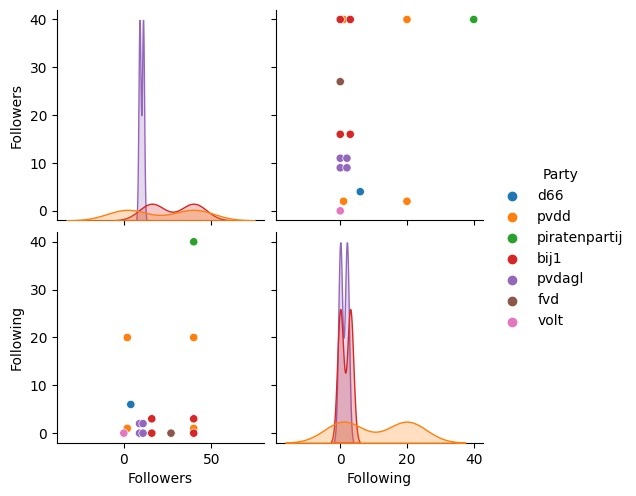
\includegraphics[width=\textwidth]{media/parties-following-counts.jpeg}
    \captionsetup{justification=centering}
    \caption{This is a subcaption}
    \label{fig:partyfollowers}
  \end{subfigure}
  \begin{subfigure}[h]{.49\linewidth}
      \captionsetup{justification=centering}
      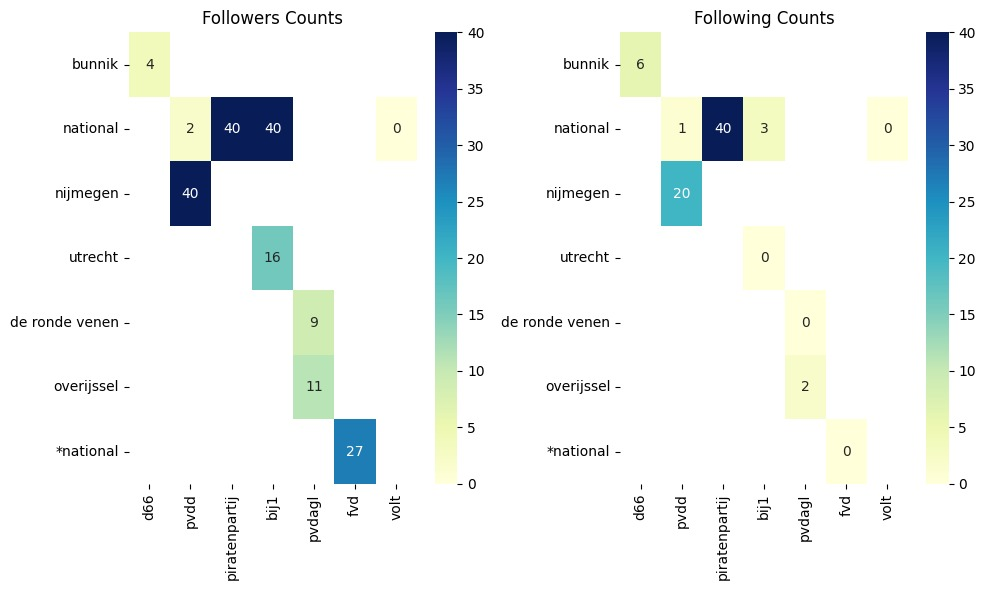
\includegraphics[width=\textwidth]{media/parties-following-region-counts.jpeg}
      \caption{This is a subcaption}
      \label{fig:partyfollowingregions}
  \end{subfigure}
  \caption{Graphs visualizing parties and follower counts}
  \label{fig:partyfollowerstotal}
\end{figure*}


\textbf{Finding M3:} \textit{Out of all parties, 7 parties are present on Mastodon and 2 have their own instances.}

\section{Discussion}

Privacy \& ethical considerations mainly for our research project on Mastodon \\ 


Besides these considerations specifically for this research, in general, it is becoming increasingly more difficult to investigate the social web and user-generated content and metadata due to several privacy scandals related to social networking platforms. Big Data Graph API's access is being heavily restricted and only available after extensive authorisation (e.g. Facebook Graph API after the Cambridge Analytica scandal \cite{cambridge}) and real-time streaming API's access is being rated limited, paywalled, or blocked entirely due to fear of AI scraping (e.g. Twitter rate limited their API \cite{Twitter}, developers need to pay for Reddit API usage \cite{reddit}).
\section{Future work}

In future work, it will be important to consider several key factors to enhance the effectiveness and enrich the datasets used in this research which are described in more detail below.

Currently, this research uses a subset of metadata available for each political party. Mainly the party names and election results. To further cross-reference the Mastodon we could enrich the metadata for each party to incorporate political spectrum data (e.g. official grouping from ProDemos or how parties voted based on the StemmenTracker \footnote{https://home.stemmentracker.nl/}) and 'weigh' each party based on left-wing, neutral or right-wing. With this the research could incorporate a 'popularity weighting' of each party since our current visualization treat each party the same not taking into account the amount of seats in the house of representatives or number of members.

The (Network) analysis currently also focusses on political parties and thus instances or servers related to the political parties but analysation of individual user accounts of faction leaders is not yet performed. To further analyse the network and get an overview of connections analysyation of personal accounts need to be performed to plot further relations of the network based on who faction leaders follow or who are following them  (e.g. handshake lemma) \cite{handshake}.

Query words and list of election-related topics in this research are manually labelled. This can be further expanded by automating this task, for example using Natural Language Processing (NLP) to scan through the table of contents of election manifestos or determine topics automatically based on keywords in quotes from voting guides. This also further enhances the reliability of the data since topics displayed in voting guides are what parties mostly disagree on. This doesn't necessarily mean these topics are the most popular topics in society among voters. For future research, it would also be interesting to cross-reference topics from the voting guides with topics discussed on social networks to see if topics that gain traction on social networking sites align with topics from voting guides.
\section{Conclusion}


The research presented in this paper delved into the dynamics of political activity on the Mastodon platform, focusing on the Dutch House of Representatives elections. The results, analyzed through three research questions, provided valuable insights into the adoption and engagement of political parties on this decentralized social network.

Firstly, the overall activity surrounding the Dutch elections on Mastodon exhibited a significant increase, particularly in the most recent election year, 2023 contrasted with minimal activity observed in the preceding elections of 2017 and 2021. The examination of the activity of political parties revealed that while a few parties dominated the discussion, the nature of their engagement varied. The Socialist Party (SP) emerged as a notable outlier, prominently featured in discussions, possibly influenced by the prevalence of their initials in the Dutch language. Interestingly, parties like the Piratenpartij demonstrated active engagement, with their own Mastodon instance, while others, like the GL-PvdA party, garnered attention despite not being directly active on the platform.

Furthermore, the analysis of election-related topics and query words highlighted the prevalence of certain themes, such as climate and the economy, predominantly associated with left-leaning parties. However, no distinct differences in discourse were observed between parties, emphasizing the even spread of discussions across various topics when parties with activity on the platform were mentioned.

Finally, the exploration of party accounts and servers revealed that a limited number of parties actively participated on Mastodon. Notably, some parties established their own instances, reflecting a commitment to decentralized structures and specialized platforms. The Piratenpartij, with its focus on internet laws and net neutrality, and Bij1, advocating for decentralized structures, exemplified this trend.

In summary, Mastodon's role in political discourse around Dutch elections has evolved, with increased activity and nuanced engagement by political parties. The findings contribute to our understanding of the dynamics of political discussions in decentralized social networks, shedding light on the platforms and strategies adopted by parties to navigate the digital social media networking landscape. With this work, we invite researchers, journalists, and practitioners alike to further investigate Mastodon in relation to the Dutch House of Representatives elections and explore any other new and upcoming Social Networking Site using similar methodology.
\section{Acknowledgements}

We thank coordinator Dr. Davide Ceolin (Vrije Universiteit Amsterdam) for providing guidance and assistance during the project and Dr. Emmanuelle Beauxis-Aussalet (Vrije Universiteit Amsterdam) who provided valuable feedback and answered our questions during the seminars which helped us further expand our research. 
\section{Conflicts of Interest}

The author(s) declared no potential conflicts of interest with respect to the research, authorship, and/or publication of this article. The author(s) has no affiliation with any of the companies and organizations mentioned in this article and this work has not been supported by any funding agency, private organization, or political party.
\section{Appendix}

In the spirit of open research in order to support reproducibility and enable future work in this problem space the datasets and Python notebooks in this work are publicly avaliable on GitHub using the MIT License. Under the \textit{dandevri} username (one of the authors) we have several a code repository with several subfolders:

\begin{enumerate}
  \item \textbf{Notebooks:} Source Code for the Python  Jupyter Notebooks for data scraping and processing. \underline{https://github.com/dandevri/vu-social-web-data/notebooks}
  \item \textbf{Datasets:} The processed and transformed datasets used in the notebooks. \\  \underline{{https://github.com/dandevri/vu-social-web-data/datasets}}
\end{enumerate}

% ---- Bibliography ----
%
% BibTeX users should specify bibliography style 'splncs04'.
% References will then be sorted and formatted in the correct style.
%
% \bibliographystyle{splncs04}
% \bibliography{mybibliography}
%

\bibliographystyle{splncs04}
\bibliography{references}

\end{document}
